%% The first command in your LaTeX source must be the \documentclass command.
\documentclass[sigconf,authorversion]{acmart}
\usepackage{pgf}
\usepackage{pgfplots}
\usepackage{url}
%% NOTE that a single column version may be required for
%% submission and peer review. This can be done by changing
%% the \doucmentclass[...]{acmart} in this template to
%% \documentclass[manuscript,screen,review]{acmart}
\providecommand{\tightlist}{%
  \setlength{\itemsep}{0pt}\setlength{\parskip}{0pt}}

\begin{document}
\settopmatter{printacmref=false}
\setcopyright{none}
\renewcommand\footnotetextcopyrightpermission[1]{}
\pagestyle{plain}
\title{Automatic Music Generation with Deep Learning}

%%
%% The "author" command and its associated commands are used to define
%% the authors and their affiliations.
%% Of note is the shared affiliation of the first two authors, and the
%% "authornote" and "authornotemark" commands
%% used to denote shared contribution to the research.
\author{Nhut Minh Phan}
\email{phan92@uw.edu}
\affiliation{%
  \institution{University of Washington}
  \city{Bothell}
  \state{WA}
  \country{USA}
}

\begin{abstract}
Automatic music generation is the art of generating new music with little human 
intervention. This art has a long history, and recently breakthrough in deep learning
provides brand-new tools for artists and untrained curious laypersons to generate
their own music with any level of music understanding. A music recording could be 
presented in different data types: raw audio waveforms, frequency-domain spectrogram, 
and symbolic representation of piano rolls. Any of these data types could be used 
to train deep learning models. This paper presents the results of experiments with 
recurrent neural networks (LSTM, bidirectional LSTM), and 1-D convolutional neural 
networks for automatic music generation. Specifically, we investigate single-track 
classical piano music generation at the musical note level. The code for preprocessing 
data and building deep learning models are available at 
\url{https://github.com/jackPhn/CSS586_Project/}.
\end{abstract}

\keywords{deep learning, neural networks, recurrent models, music}

\maketitle

\section{Introduction}

The poet Henry Wadsworth Longfellow once said that music is the universal 
language of mankind. Truely, we use music to convey emotion and feeling without
words. Music is an integral part of human culture, which
came into existence since the dawn of civilization and has since continued to 
proliferate into various forms. Composing a piece of music is a complicated process 
requiring a deep understanding of music theory and creativity. To 
generate new music, typically a composition is created in the form of music notation 
like sheet music prior to transforming it to sound by the hand of one or more musicians.
Because music generation is a specialized process that requires a lot of training,
generating music is still preserved for a trained musicians. To promote the discovery of 
new music, everyone should be able to generate their own music without spending
years of training. 

There are multiple representations of music to consider. Music data are available
as raw time-domain audio waveform, frequency-domain spectrogram, or symbolic
representation called piano rolls. A piece of music consists of one or more musical
tracks generated by one or more musicians performing on different musical
instruments.

Deep learning has been successfully used in applications ranging from speech
recognition to image classification and segmentation, among many others tasks.
The generative capacity of deep learning is recently discovered and has been
explored extensively to generate novel images, videos, and texts.
Recurrent Neural Network (RNN) has shown its capability to
model time-series sequences. Advanced version of RNN such as Gated Recurrent 
Unit (GRU) and Long Short-Term Memory (LSTM) have been successfully used for 
applications such as voice recognition, text to speech, and other applications 
that involve time-series data. RNN could also be used to generate novel 
sequences of texts or sounds. In addition to RNN, 1D convolutional neural network
could also model the dependencies between elements in a sequence.

In this paper, we investigate the use of sequential recurrent models and 1-D 
convolutional neural network to model the dependency among the notes and chords
of musical sequences from classical music performed on piano. The trained models 
are used to generate single-track piano performances.

\section{Related Work}

Automatic music generation dates back to 1781 when Mozarts invented 
a musical dice game in which a player generate new music by selecting
a tone from a list of pre-composed tone based on the sum of two dices 
\cite{enwiki:995309040}. In the past decade, deep learning has become
a increasingly popular tool for artists and researchers who are interested in automatic 
music generation. This section introduces several state-of-the-art deep learning 
works in the field of automatic music generation.

In the physical domain, a sound is essentially the displacement of air molecules,
which results in fluctuation in air pressure. When sound or music is recorded,
tens of thousands of air pressure data points are captured per second to
construct the raw audio waveform. Since a piece of music spans anywhere between 
a few seconds to several minutes, its raw audio waveform contains a large amount
of data, making the modeling of long-distance dependencies difficult. Google DeepMind
based in London, UK, introduced WaveNet, a generative deep neural network, in 2016
to tackle this problem \cite{oord_wavenet_2016}. WaveNet is a fully probabilistic
and autoprogressive model, in which the distribution of each audio sample depends on 
the previous ones. It was used to generate spoken English speech and music.

Another generative model that operates on the time-domain raw audio waveforms is 
SampleRNN \cite{mehri_samplernn_2017}. This model consists of memory-less autoregressive 
multilayer perceptron modules and stateful recurrent neural networks in a hierarchical 
structure. This combination allows the model to capture the structure of temporal 
sequences over long time spans.

Modeling raw audio waveforms is challenging since a single second in
modern recording spans thousands of timesteps. Most commonly, music is
recorded at 44.1 kHz (44,100 samples per second). Since a piece of music
is at least a few seconds in length, capturing long-range dependencies
is difficult in the time domain. A model named MelNet was introduced to address
this limitation of time-domain models \cite{vasquez_melnet_2019-1}. MelNet 
leverages a two-dimentsional time-frequency representation of audio called 
spectrogram, which reduces the dimensionality of the audio waveforms. This 
model was able to generate high-fidelity audio samples using structures on
long timescales.

The discussion on generative models is not complete without mention of Generative
Adversarial Networks (GAN). Google AI introduced GANSynth in 2019 following the 
publication of WaveNet \cite{engel_gansynth_2019}. GANSynth generates log-magnitude
spectrograms and phases prior to generating the audio waveform. It was shown to 
outperform WaveNet in automatic and human evaluations and could generate music much
faster than WaveNet.

Music creation typically starts with the composition of a musical score prior 
to the performance by a musician. The majority of works in automatic music 
generation focus on training a model using performance data like audio sound or
 its frequency transformation. Two researchers from Taiwan took another
approach and published PerformanceNet, a score-to-audio music generation model
\cite{wang_performancenet_2018}. This model consists of two subnets: a U-Net-like 
convolutional neural network that maps musical scores in the form of piano rolls 
to spectrograms; and a residual network that refines the outputs.

\section{Methods}

\subsection{Datasets}

To train our models and to provide seeds for music generation, we used 
the MusicNet, an open-source dataset published by the department of Computer 
Science at the University of Washington \cite{thickstun_learning_2017}. This 
dataset contains a collection of 330 freely-licensed classical music recordings 
captured under various studio and microphone conditions. The recordings are
available in .wav raw audio format and MIDI (Musical Instrument Digital
Interface). A MIDI file contains the encoding of music, which is not playable
like an audio file but is viewable using specialized software such as 
Apple GarageBand. It contains the performance information such as musical
instruments and the temporal location of notes and chords in a composition.

MusicNet consists of music composed by Beethoven, Bach, Ravel, Faure, and Schubert,
to name a few. Since the focus of this project is on piano music generation, only 
Schubert's compositions are selected.

\subsection{Data Preprocessing}

MIDI files are in a specialized format that requires extensive processing as 
the data are encoded according to the MIDI standard. Several open-source Python
packages exist to assist the works on MIDI files. A few examples are Pypianoroll 
\cite{dong_pypianoroll_2018} and music21 \cite{cuthbert_music21_2010}. We
decided to use music21 to process the MIDI files from Schubert's collection.

Although the main instrument used to perform the compositions in Schubert's
collection is the piano, several recordings contain musical tracks generated by 
string instruments and other instruments. Since our focus is on piano music,
these tracks need to be filtered out. To do this, the MIDI files are partitioned 
by the instruments. After partitioning, each file contains an array of different
instrument tracks. Any track other than piano is removed. 

A music21 instrument track is a Python object containing a list of notes and chords
(multiple notes played at the same time) that are played at different time points in 
a composition. It also contains rest (silence) and sustain (holding the
previous note continuously). For simplicity, the rest and sustain are discarded
from the dataset. The MIDI file format also specifies the amplitude values of 
the air pressure, which are presented in the vertical axis of a plot of the raw 
audio waveform. This information denotes the volume of each note in a performance.
For this project, the information about note volume would unnecessarily increase the 
dimensionality of the data. We decided to disregard the volume and to use the same 
pressure value for all notes and chords. 

From the isolated piano tracks, we built a corpus of extracted notes and chords. 
There is a maximum of 128 musical notes in any given piece of music. Chords, on the 
other hand, are combination of two or more notes; thus the number of possible permutations 
is very large. In Schubert's collection, the number of distinct notes and chords is 312. 
We decided to use all 312 notes and chord for single-track
piano music generation. We mapped unique integers to the notes and chords since deep 
learning models do not work well with non-numeric data format.

Each song in Schubert's collection spans a few minutes. However, our goal for this 
project is to model short sequences of music. To this end, we partitioned the corpus
into sequences of 100 notes/chords. The sequences are created by sliding a 100-note-long
window on the corpus, moving it one element at a time. The label for each sequence is 
the immediate element in the corpus that is next to its last element. 
Figure \ref{preprocessing} provides a summary for the data preprocessing pipeline.

\begin{figure}[h]
  \centering
  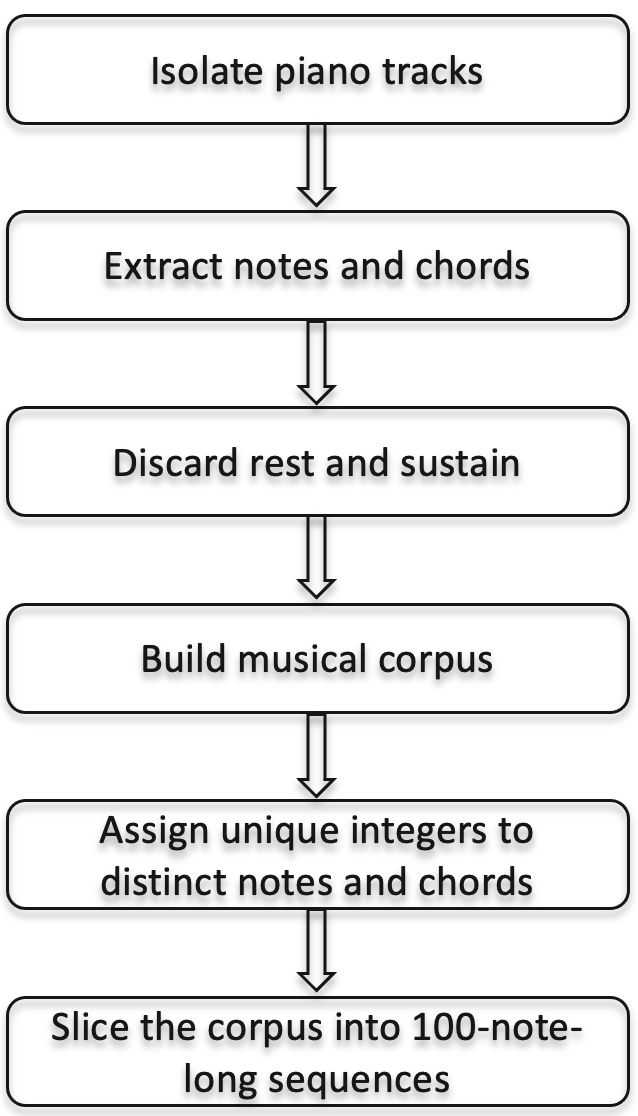
\includegraphics[width=0.5\linewidth]{preprocess.png}
  \caption{The data preprocessing pipeline consists of five steps.}
  \label{preprocessing}
  \Description{Preprocessing pipeline.}
\end{figure}

\subsection{Model Design}

In this project, we treat a short piece of music like 
a sentence, in which the vocabulary is the collection of distinct notes 
and chords, and the grammar is the local and global dependencies between
the notes and chords. We explore the effectiveness of four types of models 
in automatic music generation: Long Short Term Memory (LSTM), Bidirectional
LSTM, Bidirectional LSTM with attention, and a 1D convolutional neural 
network inspired by WaveNet's architecture. These models are many-to-one
models since the input is a sequence of multiple musical values and the output 
is a single note or chord. The models are built using the TensorFlow library.

\subsubsection{LSTM Model}

The first model is a recurrent neural network that contains LSTM layer as 
the basic building block. The LSTM model is selected because it is able to encode
the dependencies between the elements of a long sequence via a gating
mechanism. The main components of the model are LSTM layers and fully connected
layers. The output layer has 312 perceptrons corresponding to the number
of distinct musical notes and chords in the dataset. An output perceptron 
calculates the probabilities that its corresponding note or chord is the next
element in the sequence. The output activation function is softmax and the
model is trained by minimizing the sparse categorical cross-entropy loss.
The architecture of this model is shown in Figure \ref{lstm_model}.

\begin{figure}[h]
  \centering
  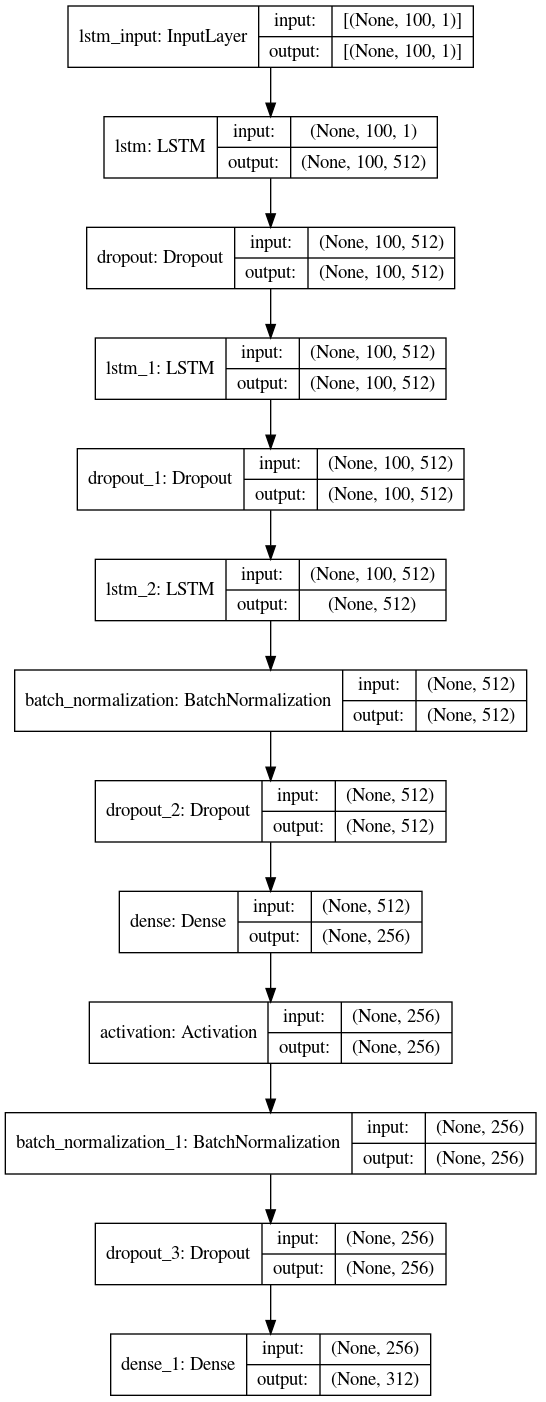
\includegraphics[width=0.6\linewidth]{lstm_model.png}
  \caption{Architecture of the LSTM model.}
  \label{lstm_model}
  \Description{LSTM model}
\end{figure}

\subsubsection{Bidirectional LSTM Model}

LSTM models capture the information in a sequence only in the forward direction,
from the beginning to end. An enhanced version of LSTM models is the bidirectional 
LSTM model. A bidirectional LSTM model trains two LSTMs simultaneously, one on the 
input sequence and another on the inverted input sequence. Effectively, the model 
encodes the structure of the past as well as the future. The bidirectional LSTM
model shares the same architecture as LSTM model, with the only difference being
the replacement of the LSTM layer by the bidirectional LSTM layer. Figure 
\ref{bidirect_lstm_model} depicts the structure of this model.

\begin{figure}[h]
  \centering
  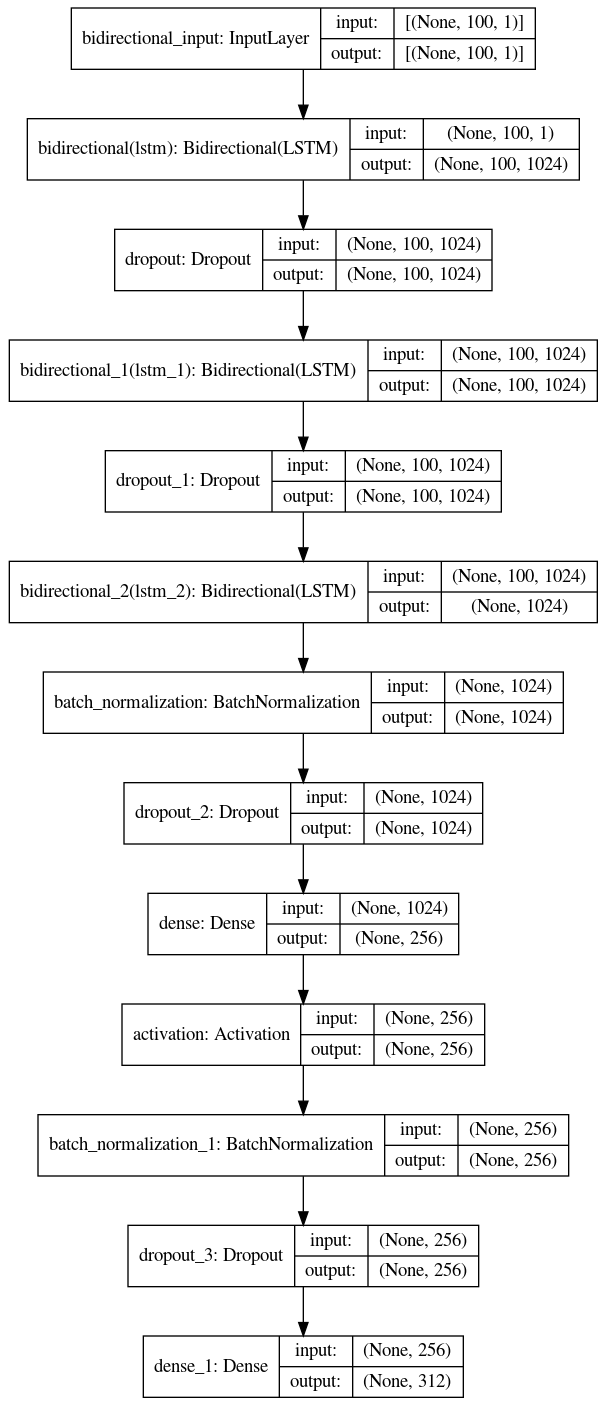
\includegraphics[width=0.6\linewidth]{bidirect_lstm_model.png}
  \caption{Architecture of the bidirectional LSTM model.}
  \label{bidirect_lstm_model}
  \Description{Bidirectional LSTM model}
\end{figure}

\subsubsection{Bidirectional LSTM Model with Attention}

The bidirectional LSTM model introduces an additional complexity by using the 
reverse of the input sequence. It is still not complete because of a fundamental
problem: its hidden states consider the elements of the input sequence with 
equal importance. To solve this problem, we added an attention layer following 
a bidirectional LSTM layer. The attention mechanism is shown in Figure 
\ref{attention_mechanism}. The importance of the hidden states of a bidirectional 
LSTM layer is captured by a set of attention weights. These weights enhance or 
supress a hidden state according to its contribution to the output of an input
sequence. Figure \ref{att_lstm_model} demonstrates how the attention mechanism
fits into the structure of the bidirectional LSTM model.

\begin{figure}[h]
  \centering
  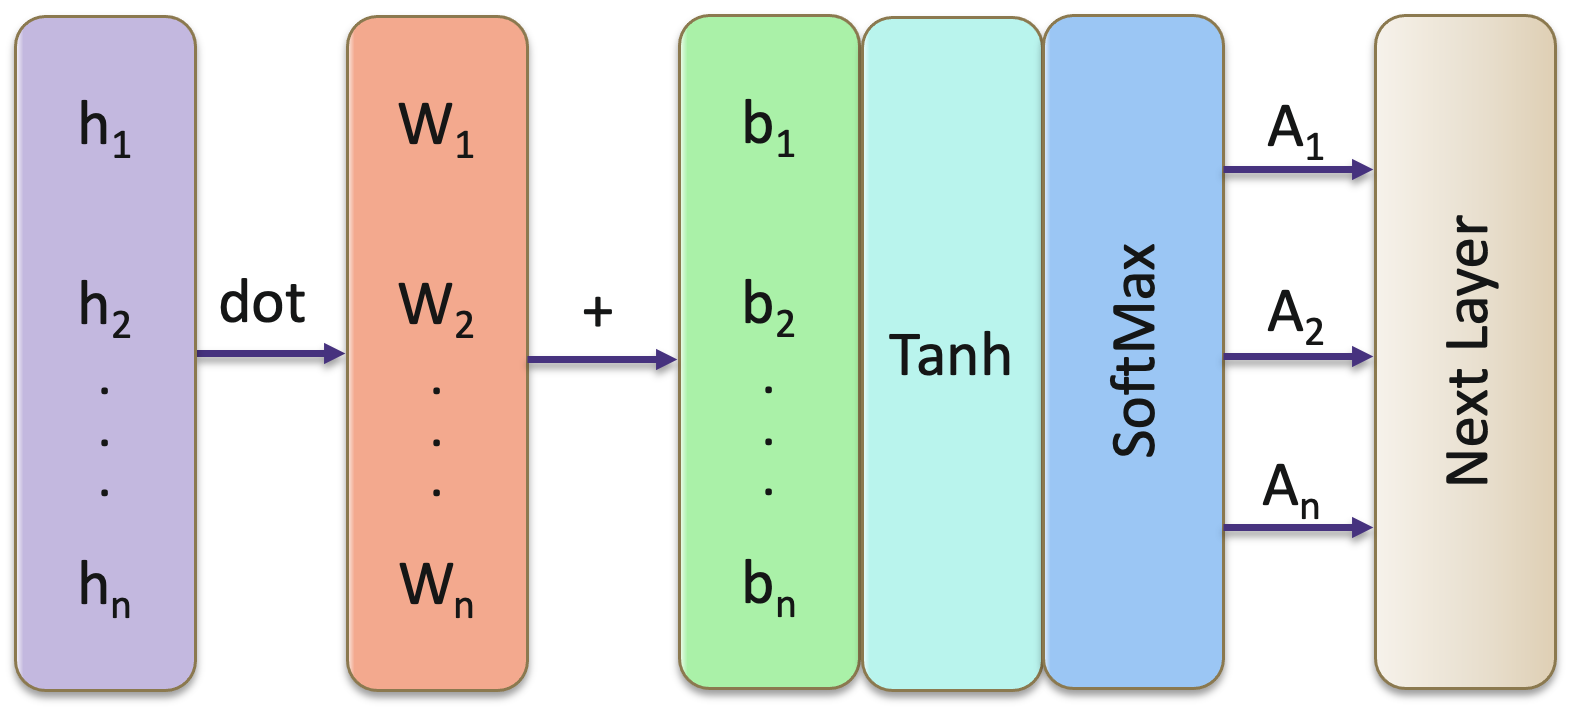
\includegraphics[width=\linewidth]{attention_mec.png}
  \caption{The attention mechanism is encapsulated in an attention block that has
  a set of attention weights (W) and attention biases (b). The attention biases are
  added to the dot product result of the previous LSTM layer's hidden state and 
  attention weights. The results are then fed into a tanh function and a softmax
  function to generate attention outputs (A).}
  \label{attention_mechanism}
  \Description{Attention mechanism.}
\end{figure}

\begin{figure}[h]
  \centering
  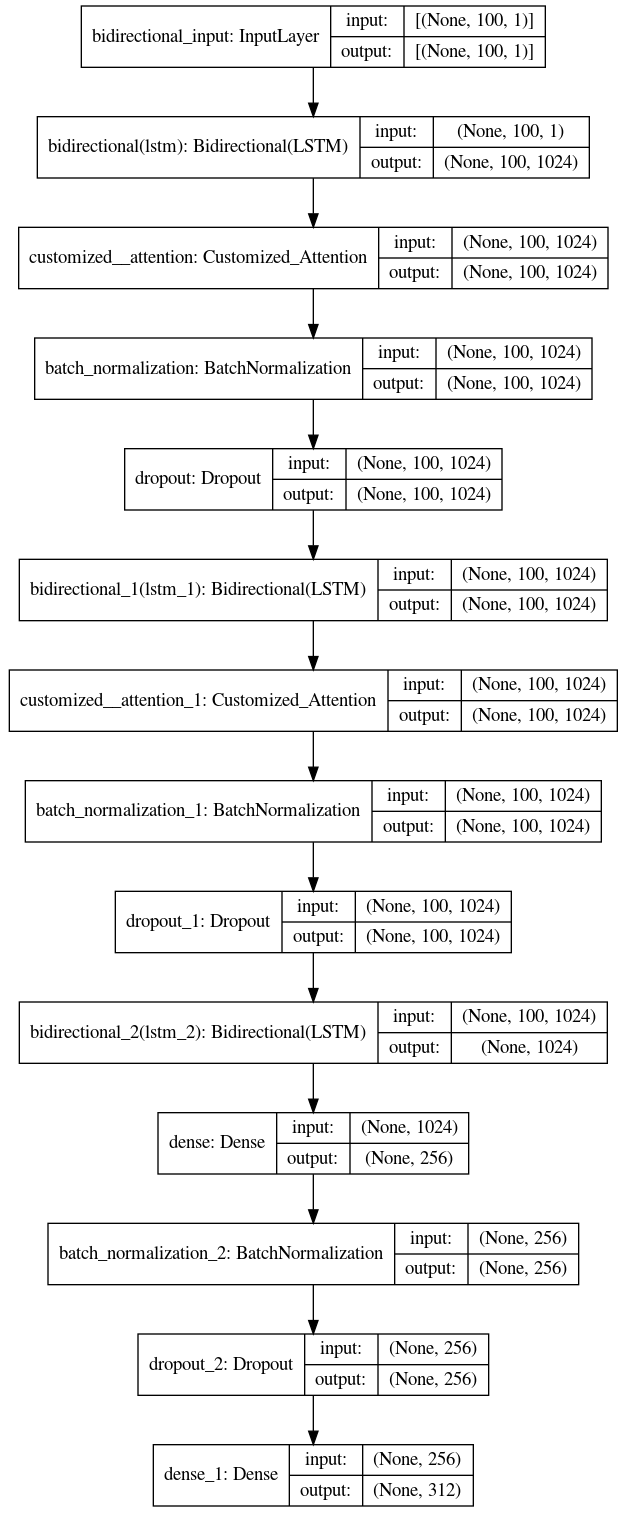
\includegraphics[width=0.6\linewidth]{attention_model.png}
  \caption{Architecture of the bidirectional LSTM model with attention mechanism.
  The Customized Attention layer is derived from Keras Layer object.}
  \label{att_lstm_model}
  \Description{Bidirectional LSTM model with attention mechanism.}
\end{figure}

\subsubsection{WaveNet-Style 1-D Convolutional Neural Network}

The original WaveNet model is designed for the raw audio waveforms, which contain
tens of thousands of discrete points per second of sound. WaveNet consists of 
 multiple 1-D dilated causal convolutional layers, which is visualized in Figure 
 \ref{causal_conv}, enabling the network to have a large receptive field. Consequently,
 the network can learn the long-term dependency in extremely long sequences. We are
 interested in this property of WaveNet and constructed our 1-D dilated causal 
 convolution network as seen in Figure \ref{wavenet_model}. The core of this network
 is three 1-D dilated causal convolutional layers that have dilation rates in ascending order 
 (1, 2, and 4). The output layer is similar to that of the LSTM models.

\begin{figure}[h]
  \centering
  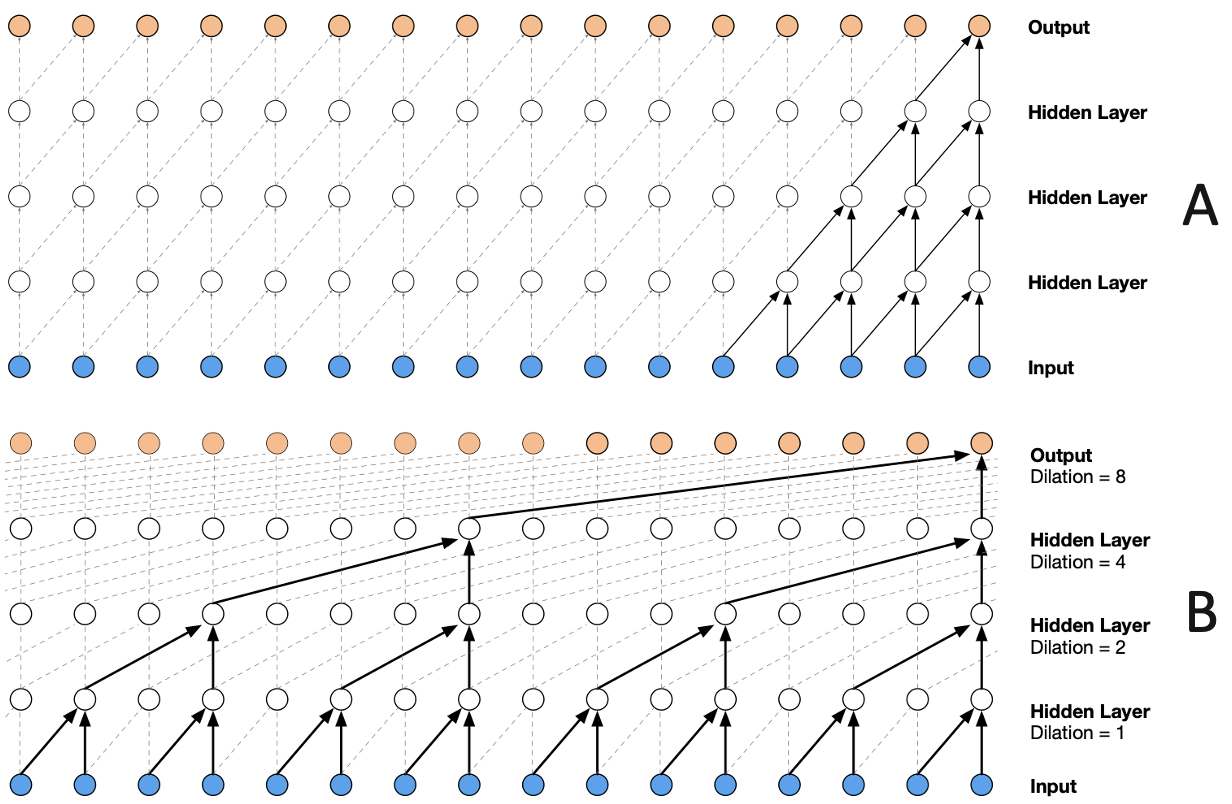
\includegraphics[width=\linewidth]{causal_conv.png}
  \caption{The core of WaveNet is dilated causal convolutuon. (A) Causal convolution 
  ensures that the output at time step t is the result of only previous time steps 
  with no input from the future. (B) With dilated convolution, the convolutional
  kernel has a larger receptive field, increasing the number of input elements
  that an output captures. Figures are adopted from the WaveNet paper \cite{oord_wavenet_2016}.}
  \label{causal_conv}
  \Description{Causal dilated convolution.}
\end{figure}

\begin{figure}[h]
  \centering
  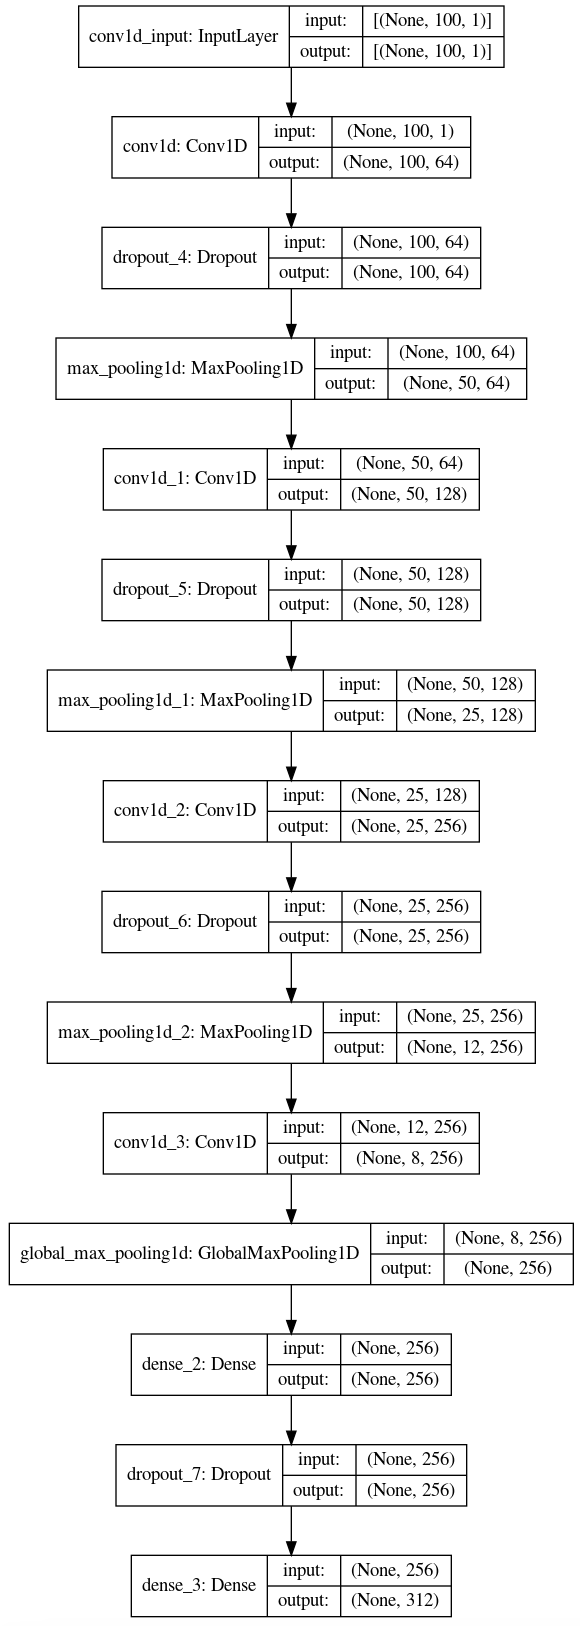
\includegraphics[width=0.6\linewidth]{wavenet_model.png}
  \caption{Architecture of the WaveNet-style 1-D dilated causal convolutional neural network.}
  \label{wavenet_model}
  \Description{Architecture of the 1D CNN.}
\end{figure}

\subsection{Generating New Music}

The same method of generating a new sequence of notes and chords is used on all trained
modules. This section describes this method, which is illustrated in Figure \ref{generate_music}. 
An input sequence containing 100 notes/chords is randomly taken from the corpus and
fed to a trained model as the initial condition. The model predicts the most probable note
or chord that comes after this input sequence. The output is appended to an output array, which is
empty at the beginning. The output note is also appended back to the input sequence. To maintain 
the input length, the first note of the input sequence is cropped out. The new input sequence
is fed into the model to gerate a new note/chord. This process is repeated until the output
array reaches a desirable length.

\begin{figure}[h]
  \centering
  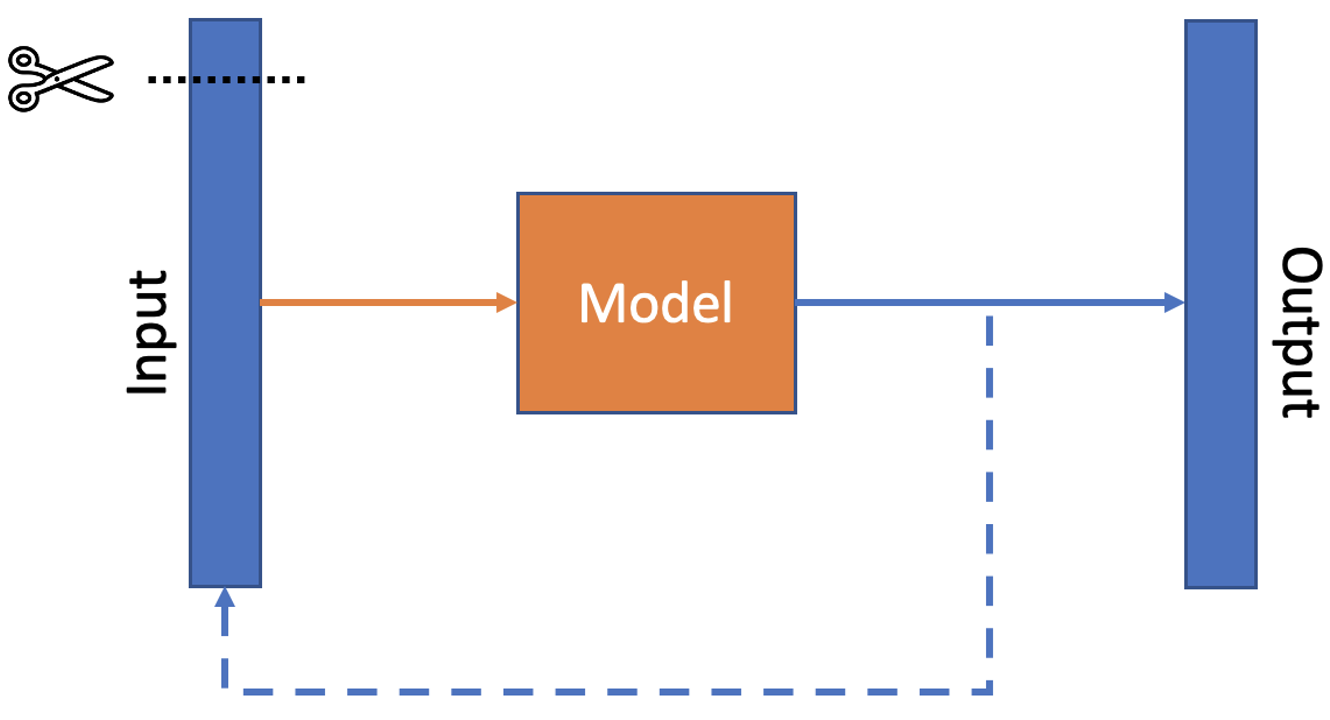
\includegraphics[width=\linewidth]{generate_music.png}
  \caption{The process of generating a new sequence of musical notes and chords 
  using an initial condition. The solid lines represent the forward path to the output
  sequence. The dashed line indicates the backward path via which the output note/chord at
  a step is appends to the end of the input sequence.}
  \label{generate_music}
  \Description{Generating music with initial condition.}
\end{figure}

\subsection{Model Evaluation}

Similar to the evaluation of GANs, evaluating music generating models is a challenging 
due to the lack of metrics that are used for supervised machine learning models.
In this paper, we evaluated the generative model by rating their outputs against our own
reference of music.


\section{Experiments and Results}

For LSTM-based models, hyperparameter tuning was performed on the basic LSTM model 
that does not have the bidirectional connection or the attention mechanism. 
The intention is that the hyperparameters that result in the best performance 
are used for the bidirectional LSTM models with and without the attention mechanism
since these more advanced models have a similar structure with the basic LSTM
model. We performed hyperparameter tuning on the following values, with the 
best parameters in \textbf{bold}:

\begin{itemize}
  \tightlist
  \item batch size: 32, \textbf{64}, 128
  \item learning rate: 0.01, \textbf{0.001}, 0.0001
  \item dimension of output space in the first LSTM layer: 64, 128, 256, \textbf{512} 
  \item dropout rate: 0.2, \textbf{0.3}, 0.4, 0.5
\end{itemize}

For the 1-D dilated causal neural network, the following hyperparameter were tested:

\begin{itemize}
  \tightlist
  \item batch size: 32, \textbf{64}, 128
  \item learning rate: 0.01, \textbf{0.001}, 0.0001
  \item number of filters in the first Conv1D layer: \textbf{64}, 128, 256
  \item number of filters in the first Conv1D layer: 64, \textbf{128}, 256
  \item number of filters in the first Conv1D layer: 64, 128, \textbf{256}
  \item number of filters in the first Conv1D layer: 64, 128, \textbf{256}
  \item number of filters in the first Conv1D layer: 64, 128, \textbf{256}
  \item dropout rate: \textbf{0.2}, 0.3, 0.4, 0.5
\end{itemize}

The models were trained for 100 epochs. After training, the models were tested by evaluating
 their generated outputs. The winning set of hyperparameters are the combinations that result
in interestingly sounding music with a lot of variations of notes and chords. Ten samples
were generated from each trained model and were assessed qualitatively. The Bidirectional
LSTM model with attention mechamism generated the most interesting outputs with lots of
variations in the notes and chords.

\section{Sample Outputs}

A collection of music generated by the LSTM models and 1-D dilated causal convolutional 
neural network is available at 
\sloppy
\url{https://drive.google.com/drive/u/1/folders/1IO3X1OMwHKwNm26uXmez6XGLeyNLG1PZ}.

\section{Conclusion and Discussion}

Automatic music generation is an interesting problem that has recently benefited from the
development of advanced machine learning techniques. Despite being in infancy,
research has shown that deep learning generative models could produce interesting music 
with little to no human intervention. In this project, we experimented with four different
deep learning architectures, LSTM, bidirectional LSTM, bidirectional LSTM with attention
mechanism, and a WaveNet-inspired 1-D dilated causal convolutional neural network. By 
qualitative evaluation, we determined that the bidirectional LSTM model with attention 
mechanism generates the most interesting pieces of music compared to the other models.
This work, although is not directly related to my partner Alex Kyllo work on generative
models for string-quartet-based classical music, demonstrates a different perspective 
on single-track piano music generation by treating a short sequence of musical notes
and chords as a written language sentence with vocabulary and grammar.

To expand upon this project, additional work is needed to search for more sophisticated
deep learning architectures that can capture the short-term, mid-range, and long-term 
dependencies among the notes of a musical composition. Furthermore, these architectures 
should be generalized to music that is performed by multiple instruments (multi-track 
polyphonic music)). Another improvement is to enable the generative models to work with
multiple musical genres, not just classical music. Finally, we only relied on our own
qualitative evaluation to assess the quality of the models due to the time constraint
of the project. We also need a comprehensive evaluation plan, which involves qualitative evaluation 
by the multiple human judges and quantitative evaluation on the structure of the generative 
musical sequences.

\bibliographystyle{ACM-Reference-Format}
\bibliography{paper}

\end{document}
\endinput
